\subsection{VQA and QNN}
\label{VQA}

Hybrid techniques involving quantum circuits and classical optimisers have been proposed to overcome the restrictions of Noisy Intermediate-Scale Quantum (NISQ) \cite{brooksQuantumSupremacyHunt2019} devices. 
Those restrictions include inability of NISQ devices to achieve fault-tolerance, restrictions on the number of the available qubits per their quantum processors, and the limited depth of practically executable quantum circuits. 
Moreover, quantum circuits and their gates are static by design, which means that input data into a quantum algorithm must be encoded as gates of the circuit implementing this algorithm. This implies that each instance of quantum algorithm use results in a new and distinct quantum circuit. This creates a barrier to using quantum circuits in support of efficient algorithm optimisation and training of quantum machine learning models.

Nevertheless, hybrid techniques, which combine classical and quantum techniques, allow development of \emph{variational circuits} (or circuit templates) with trainable parameters that can be iteratively refined by instantiating their values to create a static circuit using a traditional (classical) computer (e.g. when training VQAs) \cite{cerezo2021variational}, but which can then be efficiently executed on a quantum machine.
In this way, it is also possible to rely on range of classical optimisers, which treat variational circuits as black boxes capable of yielding outputs from inputs and the trainable parameters.

Consider a simple problem that we want to solve using VQA, given access to the training data.
The first step is to construct a \textit{cost function} $C$ used to search for an optimal set of circuit parameters, which is achieved by minimising the cost function during the training process.
We can simplify the development of variational circuits by composing the circuit templates called \textit{ansatze}. 
\textit{Ansatz} is the parameterised circuit that depends on a set of parameters $\theta$. We aim to train the ansatze by optimising the parameters $\theta$s so that the cost function $C$ reaches its minimum, thus satisfying:
\begin{equation}
    \theta^* = \underset{\theta}{\arg \min} \;C(\theta)
    \label{optimize theta with ansatz}
\end{equation}

In short, the cost function $C(\theta)$ is calculated using the quantum computer, while the classical optimiser trains the parameters $\theta$. Figure \ref{VQA diagram} explains the VQA architecture and elaborates its training process in more detail.

\begin{figure}
    \centering
    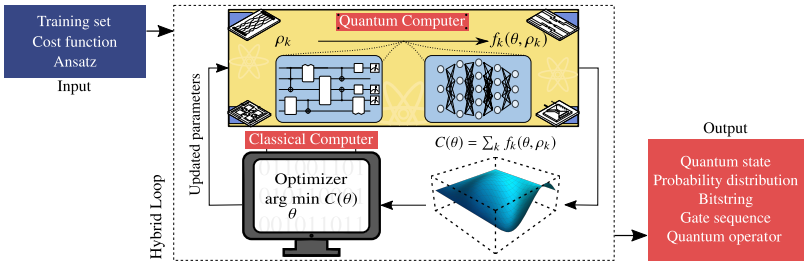
\includegraphics[width=\textwidth]{LiteratureReview/Appendices/vqadiagram.png}
    \caption{
    An illustrative diagram of VQA. 
    The algorithm is a hybrid loop that receives: 
    A cost function $C(\theta)$ for $\theta$ is a set of parameters that encodes the solution; 
    An ansatz that receives trainable parameter $\theta$ to solve the task;
    A set of training data $\{\rho_k\}$.
    We use the quantum computer to calculate the cost for each iteration, then use an optimisation algorithm in a classical computer to find the global minima in the cost landscape $C(\theta)$ and thus satisfy the problem in Eq. (\ref{optimize theta with ansatz}).
    VQA's result is an approximation of the problem solution, which can take forms as in the red box.
    Figure from Cerezo et al. \cite{cerezo2021variational}.
    }
    \label{VQA diagram}
\end{figure}

\subsubsection{The Cost Function}
Encoding the problem into a cost function is the first step in solving a problem using VQA \cite{cerezo2021variational}.
The cost function is equivalent to that used in classical machine learning. 
It maps the values of the trainable parameters $\theta$ into real values, which represent the measure of distance from an optimum solution.
For a function $f$ that receives input states $\{\rho_k\}$, observables $\{O_k\}$, and a parameterized circuit $U(\theta)$, the cost is expressed as:
\begin{equation}
    C(\theta) = f(\{\rho_k\}, \{O_k\}, U(\theta)) \;,
\end{equation}
or this form with a set of functions $\{ f_k \}$ and the square of a distance matrix given as its trace $Tr$:
\begin{equation}
    C(\theta) = \sum_k f_k \left(\Tr[ O_k U(\theta) \rho_k U^\dagger(\theta) ]\right) \;,
    \label{Cost function}
\end{equation}

For the function to be used as a cost function it must meet a number of criteria: 
(1) The cost function must be 'faithful' and 'operationally meaningful', such that the minimum of $C(\theta)$ should correspond to the solution of the problem, and the lower cost function indicate a better solution in general;
(2) Cost function must be 'efficiently estimable' by the measurement conducted on a quantum computer and the subsequent classical post-processing;
(3) The cost must be 'trainable', such that the parameters $\theta$ could be efficiently optimised.

\subsubsection{Ansatze}
\begin{figure} 
    \centerline{
        \Qcircuit @C=1em @R=0em {
        & \multigate{2}{U_1(\theta_1)}    & \multigate{2}{U_2(\theta_2)}    & \qw &        & & \multigate{2}{U_L(\theta_L)}   & \qw\\
        & \ghost{U_1(\theta_1)}           & \ghost{U_2(\theta_2)}           & \qw & \cdots & & \ghost{U_L(\theta_L)}          & \qw\\
        & \ghost{U_1(\theta_1)}           & \ghost{U_2(\theta_2)}           & \qw &        & & \ghost{U_L(\theta_L)}          & \qw
        \gategroup{1}{2}{3}{7}{.6em}{--}
        }
    }
    \centerline{$U(\theta)$}
    \centerline{}
    \centerline{}
    \centerline{
        \Qcircuit @C=1em @R=0em{
        & \multigate{1}{}   & \ctrl{2}  & \gate{}           & \qw \\
        & \ghost{}          & \qw       & \multigate{1}{}   & \qw \\
        & \gate{}           & \targ     & \ghost{}          & \qw
        \gategroup{1}{2}{3}{4}{.6em}{--}
        }
    }
    \centerline{$U_l(\theta_l)$}
    \caption{
        A diagram of a sample ansatz (above), the ansatz is a sequence of unitaries $U_l(\theta_l)$ (below).
        The unitary $U(\theta)$ receives parameters $\theta$ is expressed by $L$ layers of unitaries $U_l(\theta_l)$ for $l$ is the layer indices.
        Each $U_l(\theta_l)$ is a circuit composed of a mix of parameterised and unparametrised gates.
    }\label{Ansatz diagram}
\end{figure}

In physics and mathematics, \emph{ansatz} (plural \emph{ansatze}) is an educated guess or a starting point from which you start looking for a solution to the problem at hand. In quantum computing, \emph{ansatz} is a parameterised circuit, formed as a sequence of unitary (or "atomic") circuits, which is used as a framework for the circuit optimisation.
In general, the location of parameters $\theta$ is determined by the ansatz form and can be trained to minimise the cost.
The ansatz structure can be defined based on the problem (called 'problem-inspired ansatze') or a generic structure (called 'problem agnostic ansatze') that can be used without any relevant information available \cite{cerezo2021variational}.

The cost function in Eq. (\ref{Cost function}) encodes the parameters $\theta$ in a unitary $U(\theta)$ and applies to the input states of the circuit. 
The figure \ref{Ansatz diagram} shows that $U(\theta)$ can be expressed as a product of $L$ consecutive unitaries:
\begin{equation}
    U(\theta) = U_L(\theta_L) \cdots U_2(\theta_2) U_1(\theta_1)\;,
\end{equation}
with each layer:
\begin{equation}
    U_l(\theta_l) = \prod_m e^{-i\theta_m H_m} W_m
\end{equation}
for unparamaterized unitary $W_m$, hermitian operator $H_m$, and $\theta_l$ is the $l$-th element of $\theta$.

\subsubsection{Gradients}
After defining the cost function and a suitable ansatz, we train the parameter $\theta = \{\theta_{l}\}$ to solve the problem in Eq. (\ref{optimize theta with ansatz}) \cite{cerezo2021variational}.
The cost function gradient helps the optimiser to find the global minima. 
Consider the cost function in Eq. (\ref{Cost function}), for a unitary that parameterises rotation $e^{i \theta_l \sigma_{l}}$, where $\theta_l$ be the $l$-th element of $\theta$, $\sigma_l$ is a Pauli rotation operator. 
We can evaluate the gradient with the parameter-shift rule:
\begin{equation}
    \frac{\partial C}{\partial\theta_l}
    = \sum_k \frac{1}{2 \sin{\alpha}} 
    \left( 
        \Tr[O_k U^\dagger(\theta_+) \rho_k U(\theta_+)] 
        - \Tr[O_k U^\dagger(\theta_-) \rho_k U(\theta_-)]
    \right) \;,
    \label{Parameter-shift rules}
\end{equation}
with $\theta_{\pm} = \theta \pm \alpha e_l$, $\alpha \in \mathbb{R}$ and $e_l$ is a vector such that its $l$-th position have the value of 1, or else 0.

Essentially, we can shift the $l$-th parameter by some amount $\alpha$, and Eq. (\ref{Parameter-shift rules}) will calculate the gradient. 


\subsubsection{Optimisers}
The accuracy of VQA greatly depends on the optimisation method.
Typically, we can achieve the solution by making successive moves along the gradient direction.
This optimisation approach is within the scope of stochastic gradient descent (SGD).
One example of SGD is the ADAM optimiser \cite{kingmaAdamMethodStochastic2014}, which can vary the size of the steps taken during optimisation to produce more efficient and precise results compared to the basic SGD.


\subsubsection{About QNN}
VQA is also the most widely used method for developing Quantum Neural Network (QNN) circuits. 
As a result, QNN inevitably inherited some of VQA's features and flaws.
Many quantum machine learning models suffer from the issue of \textit{barren plateaus} \cite{zhaoReviewQuantumNeural2021} that prevent the growth of circuit depth and lead the training of parameters to a dead end.
When training a QNN framework with a large number of qubits, this phenomenon is likely to occur; the objective function becomes flat, whereby its gradient is nearly zero across a large plateau, making it nearly impossible to identify the global minimum (also defined by the zero gradient), \cite{mccleanBarrenPlateausQuantum2018, zhaoAnalyzingBarrenPlateau2021} causing inefficiency in circuit training. 
We will discuss this matter in later sections.

% Some architectures of QNN have been proposed to counter this problems, for example: 
% Quantum Tensor Neural Network (QTNN) \cite{hugginsQuantumMachineLearning2019} which achieved a balance of computational efficiency and expressive power. 
% The tensor network can reduce the required number of qubits to process high-dimensional data with powerful optimisation algorithms.
% An alternative solution is to rely on Quantum Recurrent Neural Network (QRNN) which is constructed as a parameterised circuit \cite{takakiLearningTemporalData2021}, with some qubits being initialised and measured at each step while others memorise the past data.

Many types of QNN models also suffer from the emergence of barren plateaus during their training (although for different reasons), for example in: 
Quantum Boltzmann Machines \cite{shinguBoltzmannMachineLearning2021, zoufalVariationalQuantumBoltzmann2021}, 
Quantum Perceptrons \cite{kristensenArtificialSpikingQuantum2021} and
Quantum Generative Adversarial Networks \cite{dallaire-demersQuantumGenerativeAdversarial2018, lloydQuantumGenerativeAdversarial2018}. 
It is worth noting that Quantum Convolutional Neural Networks (QCNNs) do not exhibit barren plateaus \cite{pesahAbsenceBarrenPlateaus2021}.
Thus, training convergence is more successful for QCNNs under random initialisation.

Studies have shown that Neural Network training and execution performance involving quantum machines can be significantly higher than that achievable using today's classical hardware \cite{abbasPowerQuantumNeural2021, colesSeekingQuantumAdvantage2021}. Consequently quantum neural nets may find some promising applications, for example, in breast cancer prediction \cite{liModelAlgorithmQuantuminspired2014} or image processing \cite{matsuiQubitNeuralNetwork2009}.